\documentclass{article}
\usepackage[colorlinks=true,urlcolor=blue]{hyperref}
\usepackage{graphicx}

\title{Team ``I'm part of too many teams" Proposal}
\date{}

\author{
	Raegan Lucero
	\and
	 Caleb McWilliams
	\and
	 Daniel Bartel
 }


\begin{document}
\maketitle

\section*{Goal}

This application is meant to be used to allow a user to analyze popular Tweets and craft a post for Twitter that maximizes visibility 
based on currently trending events. This will be accomplished by finding popular trends and analyzing the content of popular tweets by examining word frequency, hashtag usage, and image usage. 

\section*{Motivation}

Twitter is an interesting social network because it strips the ideas of other networks into their barest form.
The rise and fall of various trends reflects the thoughts of hundreds of millions of people.
Creating an application that can generate posts for Twitter that maximize visibility would be an interesting study in 
social networks and groupthink.

\section*{Design Rationale}

The following APIs will be used:
\begin{enumerate}
  \item[\textbullet] \textbf{WhatTheTrend} - A web service that finds popular Twitter trends \\
    \url{http://www.whatthetrend.com}
  \item[\textbullet] \textbf{Twitter} - Twitter's API will be used to search for Tweets based on a current topic \\
    \url{https://dev.twitter.com}
  \item[\textbullet] \textbf{Words API} - ``An API for the Englihs language'' - will be used for finding synonyms for rewording Tweets \\ 
    \url{https://www.wordsapi.com}
  \item[\textbullet] \textbf{Google Image Search} - will be used to find appropriate pictures for the tweet the user is posting \\
    \url{https://developers.google.com/custom-search/json-api/v1/overview}
\end{enumerate}
	
\section*{Technical Details}

\subsection*{Implementation}
The application will be a single-page \textbf{AngularJS} application served running on a server using the \textbf{Flask} web microframework.
The GitHub repository is located here: \url{https://github.com/dbartel/csce438}.

\subsection*{Workflow}

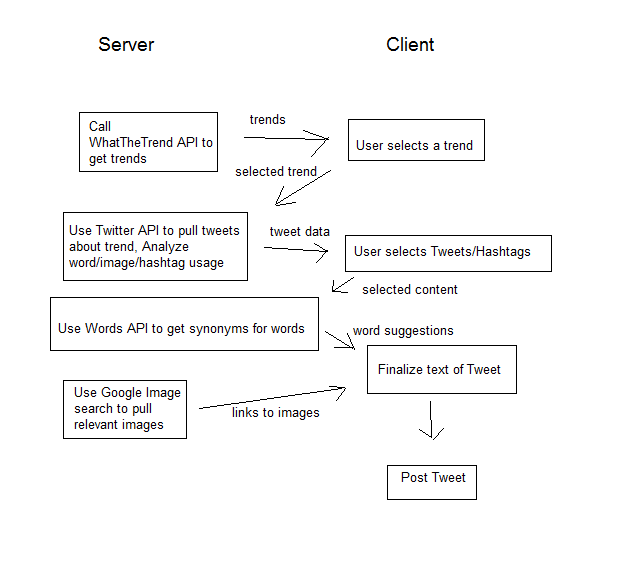
\includegraphics{diagram.png}


\end{document}
